\vspace{-15pt}
\section{Identifying and removing bias in datasets}\label{sec:sup_bias}

In this section we provide qualitative examples showing the explanations from the two models trained for distinguishing doctors from nurses- model1 which was trained on images (with an inherent bias) from a popular search engine, and model2 which was trained on a more balanced set of images from the same search engine.

As shown in \reffig{fig:sup_bias}, \gcam{} visualizations of the model (model1) predictions show that
the model had learned to look at the person's face / hairstyle to distinguish nurses from doctors, thus learning a gender stereotype.

Using the insights gained from the \gcam{} visualizations, we balanced the dataset and retrained the model. The new model, model2 not only generalizes well to a balanced test set, it also looks at the right regions, as can be seen in \reffig{fig:sup_bias}.
\begin{figure}[ht!]
\vspace{20pt}
  \begin{center}
    \begin{subfigure}[b]{0.32\linewidth}
        \centering
        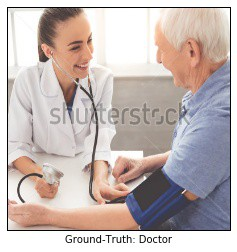
\includegraphics[width=1\linewidth]{figures/71_orig_balanced.jpg}
		\caption{\tiny{Original Image}}
        \vspace{10pt}
    \end{subfigure}
    \begin{subfigure}[b]{0.32\linewidth}
        \centering
        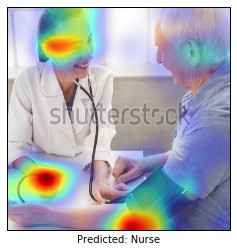
\includegraphics[width=1\linewidth]{figures/71_gcam_incorr_unbalanced.jpg}
		\caption{\tiny{\gcam{} for biased model}}
        \vspace{10pt}
    \end{subfigure}
    \begin{subfigure}[b]{0.32\linewidth}
        \centering
        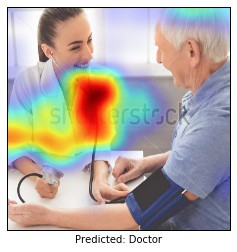
\includegraphics[width=1\linewidth]{figures/71_gcam_corr_balanced.jpg}
		\caption{\tiny{\gcam{} for unbiased model}}
        \vspace{10pt}
    \end{subfigure}
    \begin{subfigure}[b]{0.32\linewidth}
        \centering
        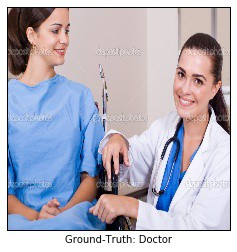
\includegraphics[width=1\linewidth]{figures/teaser/25_orig_balanced.jpg}
		\caption{\tiny{Original image}}
        \vspace{10pt}
    \end{subfigure}
    \begin{subfigure}[b]{0.32\linewidth}
        \centering
        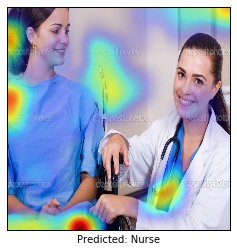
\includegraphics[width=1\linewidth]{figures/teaser/25_gcam_incorr_unbalanced.jpg}
		\caption{\tiny{\gcam{} for biased model}}
        \vspace{10pt}
    \end{subfigure}
    \begin{subfigure}[b]{0.32\linewidth}
        \centering
        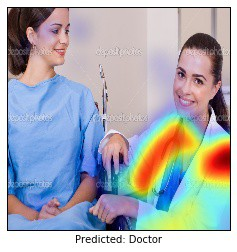
\includegraphics[width=1\linewidth]{figures/teaser/25_gcam_corr_balanced.jpg}
		\caption{\tiny{\gcam{} for unbiased model}}
        \vspace{10pt}
    \end{subfigure}
    \begin{subfigure}[b]{0.32\linewidth}
        \centering
        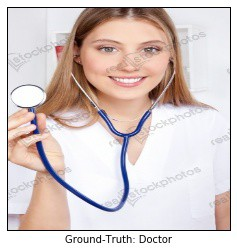
\includegraphics[width=1\linewidth]{figures/teaser/60_orig_balanced.jpg}
		\caption{\tiny{Original Image}}
        \vspace{10pt}
    \end{subfigure}
    \begin{subfigure}[b]{0.32\linewidth}
        \centering
        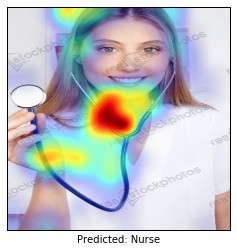
\includegraphics[width=1\linewidth]{figures/teaser/60_gcam_incorr_unbalanced.jpg}
		\caption{\tiny{\gcam{} for biased model}}
        \vspace{10pt}
    \end{subfigure}
    \begin{subfigure}[b]{0.32\linewidth}
        \centering
        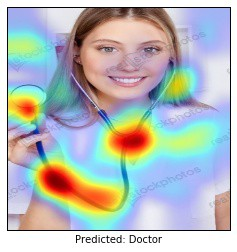
\includegraphics[width=1\linewidth]{figures/teaser/60_gcam_corr_balanced.jpg}
		\caption{\tiny{\gcam{} for unbiased model}}
        \vspace{10pt}
    \end{subfigure}
    \vspace{10pt}
	\caption{\ijcv{\gcam{} explanations for model1 and model2. 
    In all the 3 examples we see that the biased model was looking at the face of the person to predict `nurse' incorrectly, whereas the unbiased model looks at the stethoscope and the white coat to correctly predict `doctor'.}
    }
    \label{fig:sup_bias}
    \end{center}
    \vspace{-15pt}
\end{figure}